\documentclass[ProofPDF]{./Styles/Jnls-Template-V3}

% --- Optional packages (keep only what you need; the class may already load some of these) ---
\usepackage[utf8]{inputenc}
\usepackage{natbib}
\usepackage{graphicx}
\usepackage{amsmath}
\usepackage{amssymb}
\usepackage{hyperref}
\usepackage{url}

\begin{document}

% --- Journal metadata (fill in as appropriate for the journal/issue) ---
\jname{Journal Title} % TODO: replace with the journal name
\jvol{00}
\jissue{00}
\jmonth{season}
\jyear{xxx}
\jid{doi}
\artid{xx.xxxx/xxxx.xx}
\filename{Tellus\_Perspective\_Salter}
\def\MSFirstPage{\pageref{startPage_Label}}
\def\MSLastPage{\pageref{endPage_Label}}
\graphicspath{{./Images/}}
\label{startPage_Label}

% --- Article front matter ---
\title{Bubbles, Droplets, Climate: Tellus's Enduring Influence on Sea Spray Aerosol Research}

\articletype{PERSPECTIVE ARTICLE}

\author[1]{Matthew E. Salter}
\howtociteauthor[1]{Salter ME}
\rhauthor[1]{M. E. Salter}

% TODO: Replace with your actual affiliation(s) and email(s)
\aff[1]{Affiliation to be added (e.g., department, institution, city, country). \href{mailto:email@domain.com}{email@domain.com}}

\afflnote{*Author affiliations can be found in the back matter of this article}

\begin{history}
\submitted{\submittedday{xxx}\submittedmonth{xxx}\submittedyear{xxx}}
\accepted{\acceptedday{xxx}\acceptedmonth{xxx}\acceptedyear{xxx}}
\published{\publishedday{xxx}\publishedmonth{xxx}\publishedyear{xxx}}
\end{history}

\begin{abstract}[ABSTRACT]
Sea spray aerosol (SSA) is an important aspect of air-sea exchange. It influences atmospheric chemistry, cloud formation, biogeochemical cycling, and the long-range transport of both natural and anthropogenic material. A number of early studies on SSA were published in \textit{Tellus}, including the first direct evidence that bursting bubbles at the ocean surface generate particles. Critically, these foundational studies, which reach across the fields of bubble physics, interfacial chemistry, and air-sea interaction, initiated decades of subsequent research.
In this perspective article, I outline how the results of these studies have led to todays mechanistic understanding of SSA production. I document key developments, from the demonstration of jet and film drop formation, through the recognition that selective chemical fractionation occurs during bubble bursting, to modern field techniques that link the physical, chemical, and biological drivers of SSA production. I also highlight the emergence of mesocosm systems, advanced analytical methods, and dedicated wave-channel facilities, which have enabled a molecular-level understanding of nascent SSA composition, including the transfer of surface-active pollutants such as perfluoroalkyl acids.
Throughout the article, I examine how insights from the field, which trace their origins to early \textit{Tellus} publications, help frame a number of understanding challenges. These include quantifying size-resolved SSA emissions in a changing climate, assessing the role of microbial and biogeochemical processes in influencing different aspects of SSA production, and constraining the climatic relevance of SSA. The latter is particularly pertinent given the increasing interest in marine cloud brightening. By revisiting the trajectory from early \textit{Tellus} studies to present-day research, this contribution underscores the journals continuing influence on air–sea interaction science and outlines opportunities for future SSA studies.
\end{abstract}

\begin{keyword}[KEYWORDS:]
Sea spray aerosol; air--sea exchange; bubble bursting; Tellus; aerosol--cloud interactions
\end{keyword}

\maketitle

% --- Main text ---
When I was invited to write this perspective on \textit{Tellus} and its influence on air–sea interaction research, I felt both a sense of privilege and responsibility. As a researcher who has dedicated the last two decades to this field, I recognise the importance of doing justice to the pioneering studies that established its foundations. Since its inception, \textit{Tellus} has published numerous seminal papers across the broad scope of research defining this field, from the early studies that established the physical foundations of air–sea gas exchange and the ocean's role in regulating atmospheric CO$_2$
\citep{Revelle1957,Bolin1960,Broecker1974} to later advances coupling these insights with biogeochemical and isotopic perspectives on the global carbon cycle \citep{Krakauer2006}.

I am, however, perhaps best known for my work on sea spray aerosol (SSA), and it is here that I will focus this reflection. This focus is fitting, as SSA production is one of the principal pathways through which air–sea exchange occurs: bubbles generated by wave breaking mediate the transfer of gases, heat, and momentum between the ocean and atmosphere, while also scavenging dissolved and particulate material from the surface ocean. When these bubbles burst, they eject droplets that become airborne particles, linking physical hydrodynamics to atmospheric chemistry and ultimately to climate.

In what follows, I revisit how research published in \textit{Tellus} has shaped our understanding of SSA, from the first photographic evidence of bursting bubbles to the evolving recognition of their biogeochemical and climatic significance, and I reflect on how these foundations continue to inform the field’s future directions.

\section{Early Foundations: The Jet Drop Mechanism}

Given the breadth of SSA research today, it is easy to overlook how the field began and how pivotal early \textit{Tellus} papers were in defining its direction. More than 150 years have passed since \cite{Beck1819}, \cite{Sigerson1870}, and \cite{aitken1881} first suggested that the ocean could itself be a source of atmospheric particles. Their ideas began to gain wider scientific attention only after \cite{jacobs1937} identified air bubbles as the mechanism capable of producing sea-salt aerosol. By the mid-twentieth century, the prevailing view held that bursting bubbles at the sea surface were the primary source of marine aerosol, but the detailed physics of droplet formation remained unresolved.

That gap was decisively addressed by Kientzler, Arons, Blanchard, and Woodcock (\citeyear{Kientzler1954}) in their landmark \textit{Tellus} paper,\textit{Photographic Investigation of the Projection of Droplets by Bubbles Bursting at a Water Surface}. Using still photographs with $\sim 30~\mu\text{s}$ exposures and high-speed motion pictures (~3,000 fps), they captured the collapse of a bubble cavity and the formation of a narrow jet capable of ejecting droplets several diameters above the surface (see Figure~\ref{fig:kientzler_bubble_burst}). Upon evaporation, these droplets yielded salt residues matching the smallest particles observed in marine air \citep{woodcock1952}, providing the first direct mechanistic link between bubble bursting and atmospheric sea-salt aerosol.

\begin{figure}[tb]
	\processfigure
	{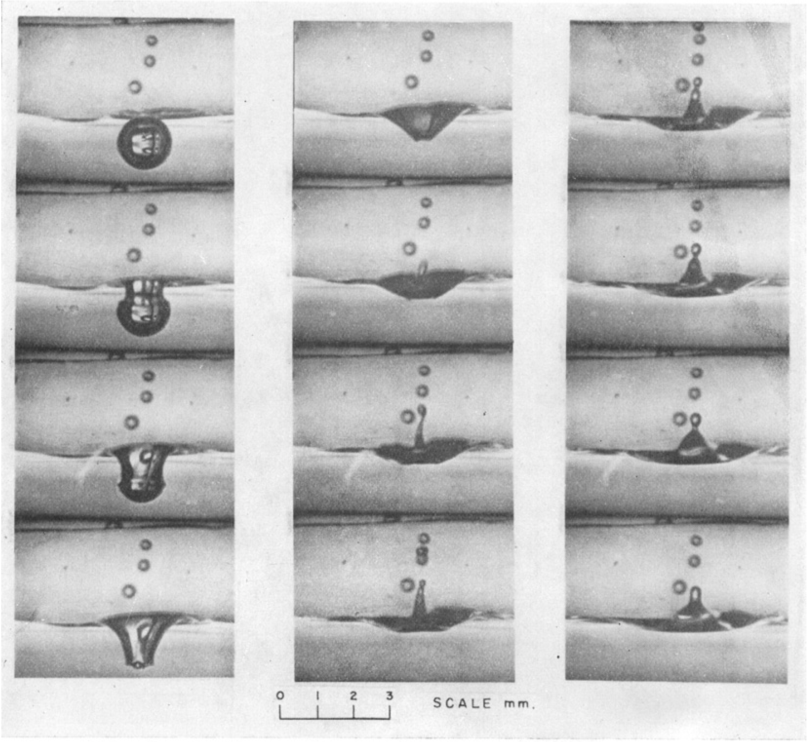
\includegraphics[width=\textwidth]{images/Kientzler_Figure_2.pdf}}
	{High-speed motion pictures of bubble bursting dynamics, reproduced from \citet{Kientzler1954}. Sequence shows 1.5 mm diameter bubbles bursting in fresh water with a clean surface, captured horizontally through a glass microscope slide. The images were taken at 3,340 frames per second, revealing the progressive stages of bubble cavity collapse and jet formation.\label{fig:kientzler_bubble_burst}}
	{Source text}
\end{figure}


Kientzler and colleagues also introduced the empirical “10\% rule,” which states that the average droplet radius is approximately one-tenth the radius of its parent bubble. This simple geometric relationship transformed qualitative observations into a quantitative framework, allowing aerosol fluxes to be estimated from measurable bubble-size distributions. Although later work refined this scaling to account for viscosity, surface tension, and film dynamics, the principle remains fundamental to understanding how bubble-scale dynamics give rise to airborne sea-salt particles \citep{Blanco2020,Wang2017}.

\section{Beyond the Jet: Emerging Chemical and Interfacial Complexity}

Although the work of \cite{Kientzler1954} clarified the physics of jet-drop formation, it left open the question of how smaller droplets arise during film rupture. Their experiments primarily captured jet drops with radii of about 20--200 $\mu$m, large enough to settle quickly and therefore unable to explain the abundant submicron sea-salt aerosol observed in the marine boundary layer. This gap was addressed in another seminal \textit{Tellus} paper, \cite{Blanchard1957}, \textit{Bubble Formation and Modification in the Sea and Its Meteorological Significance}. Their study extended the mechanistic framework by examining natural bubble-generation processes such as whitecaps, rainfall, and gas supersaturation, and by analysing how bubble dissolution and modification affect the resulting droplet-size distribution (see Figure~\ref{fig:blanchard_bubble_size}).

\begin{figure}[tb]
	\processfigure
	{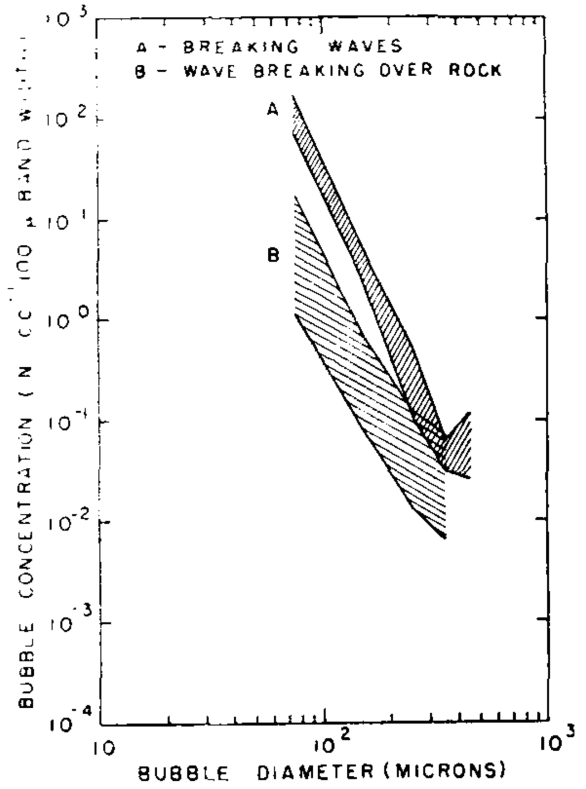
\includegraphics[width=\textwidth]{images/Blanchard_Figure_4.pdf}}
	{Bubble concentration (cc$^{-1}$ per 100 $\mu$
		band width) in seawater produced by breaking waves. Data shows bubble concentrations from different wave conditions: breaking waves on the open sea (Region A) and waves breaking over a rock (Region B), demonstrating the variability in bubble production mechanisms.\label{fig:blanchard_bubble_size}}
		{From \citet{Blanchard1957}.}
\end{figure}

Crucially, Blanchard and Woodcock moved beyond a purely physical description to incorporate the chemical and electrical properties of the emitted droplets. They observed that jet drops, often carrying appreciable charge and enriched in biological material, differ fundamentally from film drops, which are smaller, chemically distinct, and typically contain the highest fraction of organic matter. This recognition reframed the central problem: the number, size, and composition of airborne sea-salt aerosol are controlled not only by bubble dynamics but also by surface chemistry and biological modification. At the time, these observations were pioneering but not yet widely appreciated, and their relevance to air–sea exchange became evident only gradually.

\section{The Whitecap Era: From Observation to Parameterisation}

Recognising that droplets ejected from the sea surface contain more than water and salt marked a major turning point in our understanding of air–sea exchange. As early as the 1940s, \citet{Woodcock1948} reported that respiratory irritation during "red-tide" events was associated with aerosolised material from seawater enriched in dinoflagellates. Despite this early evidence that biological material could be transferred to the atmosphere, the prevailing view still held that sea spray aerosols consisted only of salt and water. This perspective shifted decisively with the work of Blanchard and colleagues, who showed through laboratory and field experiments that surface-active organic compounds are efficiently transferred into the atmosphere by bubble bursting \citep{Blanchard1963,Blanchard1964}. Their results revealed a direct chemical and biological connection between the ocean surface and airborne particles, establishing the conceptual basis for a new line of research into the partitioning of specific chemical species across the air–sea interface.

In the following decade, attention turned to "fractionation", the apparent selective enrichment of certain elements and compounds in sea spray aerosol relative to bulk seawater \citep{Macintyre1970,Barker1972,Duce1976}. Early studies suggested that bubble bursting might preferentially eject ions such as magnesium, calcium, or potassium, leading to hopes that aerosol composition could provide clues to bubble dynamics and interfacial chemistry \citep[e.g.][]{Komabayasi1964}. Although later work identified sampling artefacts in many of these observations, the experiments confirmed that bubble bursting is a highly efficient pathway for transferring organic carbon from the ocean to the atmosphere \citep{Barker1972,Duce1976,Hoffman1977}. As a result, sea spray research expanded beyond its physical roots to include the coupled biogeochemical and chemical processes linking ocean ecology with atmospheric composition and climate.

\section{The Whitecap Era: Empirical Parameterisations}

By the 1980s, the physical, chemical, and biological complexity of SSA was broadly recognised, but integrating these insights into predictive models remained a major challenge. Building on the hypothesis of \citet{Blanchard1963}, that aerosol production scales with whitecap coverage, Monahan and colleagues developed the first empirical SSA source functions based on controlled "whitecap simulation" experiments. Their formulation \citep{Monahan1986} provided a practical means to estimate global SSA emissions using wind speed and whitecap fraction as predictors, and it quickly became the standard approach for representing SSA production in climate models.

This parameterisation, however, was dominated by coarse-mode salt fluxes and thus obscured the smaller, organic-rich particles emphasised in earlier laboratory and field work. By framing SSA production primarily in terms of these larger particles, the Monahan model successfully captured the dominant salt component but not the number distribution that governs aerosol–cloud interactions. The subsequent shift toward number-based source functions and the inclusion of organic enrichment reconnected the modelling framework to the biogeochemical and microphysical processes first explored in \textit{Tellus}.

\section{Revisiting the Fine Mode: Organic Enrichment and Seasonality}

By the turn of the century, emerging theoretical and observational approaches revived long-standing questions about the chemical heterogeneity of SSA first posed by Blanchard and colleagues. Two complementary advances transformed our understanding of SSA composition: (1) the development of mechanistic models that explained the microscale processes governing aerosol heterogeneity, and (2) new field and analytical techniques that revealed direct biological modulation of aerosol composition.

On the theoretical front, researchers began to formulate mechanistic explanations for the size-dependent chemical composition of marine aerosols, first hinted at in earlier studies. \citet{Oppo1999} introduced a thermodynamic model in which an organic surface film enriches smaller droplets more strongly than larger ones, while \citet{Ellison1999} proposed a complementary view of marine aerosol particles as aqueous cores encapsulated by organic surface layers of biological origin. Although simplified, these models established the first quantitative framework linking microscale interfacial processes to aerosol composition and laid the foundation for later process-based approaches, such as competitive Langmuir adsorption frameworks, that now connect ocean biogeochemistry directly to emission parameterisations \citep[e.g.][]{Burrows2014}.

Simultaneously, advances in field and analytical capability, particularly the combination of long-term coastal monitoring, size-resolved chemical analyses, and satellite chlorophyll-a correlation, provided detailed observational evidence of biologically modulated aerosol composition \citep{odowd2004}. Measurements at coastal observatories, such as Mace Head, Ireland, showed that submicron SSA contained 60–85 \% organic matter by mass during periods of high biological activity, with total organic carbon contributing up to 83 \% in the fine mode (0.06–0.125 $\mu$m) compared with the salt-dominated aerosols of winter \citep{odowd2004}. This organic material was largely water-insoluble, indicating a primary, bubble-mediated source linked to the sea-surface microlayer and surface-ocean biology \citep{Facchini2008}. The recognition that organic enrichment is both size-dependent and biologically controlled marked a conceptual reconvergence between the physical "whitecap" framework and the biogeochemical complexity that early \textit{Tellus} papers first illuminated. These results, in turn, motivated the development of biologically modulated source functions using chlorophyll-a as a proxy for surface-ocean productivity \citep{odowd2008,Russell2010}.

\section{From Legacy to Mechanistic Synthesis: The Last Two Decades}

The publication of \citet{odowd2004} marked a defining moment in SSA research. What began in \textit{Tellus} as a question of bubble physics and droplet ejection had, by the mid-2000s, evolved into a problem of chemical complexity and biological control \citep{DeLeeuw2011}. This realisation initiated a new era of process-based inquiry, one concerned not only with how much SSA is emitted, but also with what it is composed of, how it forms, and why it varies \citep{Quinn2015}. Analytical advances soon allowed researchers to identify the molecular signatures of organic matter in SSA, including polysaccharides, proteins, lipids, and gel-like colloids, most of which were traced to the sea-surface microlayer \citep{Bertram2018}.

With the chemical complexity of nascent SSA firmly established, attention turned to quantifying how ocean biology shapes its composition. Researchers sought to determine how variations in surface-ecosystem state, from bloom conditions to oligotrophic waters, influence the quantity and character of aerosolised organic matter. Numerous investigations have since examined these links \citep[see review by][]{Bertram2018}, leading to two broad perspectives. One group of studies reported a strong dependence of SSA organic enrichment on biological activity, with elevated organic-carbon-to-sodium ($\text{OC}/\text{Na}^+$) ratios during periods of high phytoplankton biomass or bloom conditions \citep[e.g.,][]{odowd2004,Facchini2008,odowd2015}. Supporting this view, observations at sites such as Mace Head showed that the water-insoluble organic-matter (WIOM) fraction of submicron aerosol increased markedly during bloom periods \citep{odowd2004}, a pattern echoed by \citet{VanPinxteren2017} in the North Atlantic under high-chlorophyll-a conditions.

In contrast, other studies have found little or no systematic variation in $\text{OC}/\text{Na}^+$ ratios between oligotrophic and productive regimes \citep[e.g.,][]{Russell2010,Quinn2014} or in mesocosm experiments simulating bloom cycles \citep{Jayarathne2016}. These results point to an alternative interpretation: in many oceanic settings, the large and persistent reservoir of dissolved and colloidal organic carbon exerts the dominant control on SSA composition, masking the influence of local biological variability \citep[e.g.,][]{Beaupre2019}.

Global and regional datasets have sharpened this debate. Measurements from the North Atlantic Aerosol and Marine Ecosystem Study (NAAMES) revealed that seasonal variability in plankton ecosystems had little effect on either the organic fraction or cloud-condensation-nuclei (CCN) activity of freshly emitted SSA \citep{Bates2020}. Complementary results from the Atmospheric Tomography (ATom) mission extended this picture globally, showing that submicron SSA organic-mass fractions over the remote Atlantic and Pacific Oceans were typically below 10 \% in the marine boundary layer and exhibited weak seasonal variability \citep{Lawler2024}. Together, these findings suggest that in remote regions, biological control of nascent SSA composition is limited, with organic enrichment largely reflecting the background pool of dissolved organic matter \citep{Beaupre2019}.

Reconciling these perspectives, strong local biological influence versus global background control, has become one of the field’s central challenges. Addressing it requires experiments that isolate biological and physical drivers under reproducible conditions. Mesocosm studies, in which microbial communities are cultivated under controlled settings, have demonstrated direct causal links between plankton-bloom dynamics, organic-exudate production, and aerosol emissions \citep[e.g.][]{Prather2013,Lee2015}. These experiments confirmed that microbial activity and surface-active organic compounds influence not only particle concentration but also chemical composition. Subsequent laboratory work further refined this picture, distinguishing between film and jet drops and showing that film drops, which are responsible for submicron aerosols, are preferentially enriched in organic surfactants and other surface-active species \citep{Wang2017}.

Beyond natural organic surfactants, recent work has shown that SSA also serves as an efficient pathway for the atmospheric transfer of persistent anthropogenic pollutants. Laboratory studies have been instrumental in establishing that perfluoroalkyl acids (PFAAs), a class of highly surface-active contaminants, are strongly enriched in nascent SSA. Enrichment factors (EFs) relative to bulk seawater have been found to exceed $10^5$ in some cases \citep[e.g.][]{Johansson2019,Sha2020}. Complementary field observations, including measurements along the Norwegian coast \citep{Sha2021} and across the Atlantic Ocean \citep{Sha2024}, have confirmed that PFAAs are consistently enriched in SSA. Recent work has also demonstrated that SSA can aerosolise coastal water pollution more broadly, including both chemical contaminants and microbial agents, with implications for environmental fate and public health \citep{Pendergraft2023}.

The need for controlled, mechanistic studies has driven the development of a new generation of laboratory and field-deployed systems that effectively bring the ocean into the laboratory. Studies now employ diverse methods to generate nascent SSA under contamination-free conditions, including sintered-glass frits \citep[e.g.][]{Maartensson2003,Sellegri2006}, pressurised atomisers \citep[e.g.][]{Svenningsson2006}, impinging jets \citep[e.g.][]{Salter2014}, plunging waterfalls \citep[e.g.][]{Stokes2013}, and mechanically generated breaking waves \citep[e.g.][]{Prather2013}. Each approach offers distinct advantages, together forming a methodological toolbox for probing the coupled physical, chemical, and biological processes that govern aerosol production.

Comparative studies have been central to this effort. They allow systematic evaluation of the physicochemical differences among generation schemes and show, for instance, that plunging-jet and mechanically generated breaking-wave systems most closely reproduce the bubble-size distributions and aerosol properties characteristic of natural wave breaking \citep[e.g.][]{Collins2014}. Despite this, simpler devices such as sintered-glass frits and atomisers remain widely used because of their adaptability for shipboard applications, including the Sea Sweep and related onboard bubble generators \citep[e.g.][]{Bates2012}, as well as their simplicity to operate in the laboratory. Facilities such as the Marine Aerosol Reference Tank (MART) \citep{Stokes2013} and its derivatives (e.g., miniMART \citep{Stokes2016}) apply the pulsed-plunging-waterfall technique to create controlled, repeatable analogues of breaking waves. These specialised systems provide an unprecedented opportunity to connect SSA production with physical factors (e.g., sea-surface temperature, air-entrainment rate), chemical partitioning (organic speciation, mixing state), and biological properties (microbial activity, plankton dynamics).

The mechanistic perspective enabled by these systems has also refined the understanding of the inorganic fraction of SSA. Divalent cations such as calcium and magnesium have been shown to be preferentially incorporated into smaller droplets, suggesting subtle chemical fractionation during bubble bursting, an echo of the fractionation debates that animated the field in the 1960s and 1970s \citep{Salter2016,Jayarathne2016}. Whereas earlier investigators debated whether such effects reflected artefacts or bubble dynamics, modern analytical techniques have confirmed that they arise from genuine interfacial processes \citep{Schill2018,Carter2021}. These results have broadened SSA research from physical descriptions toward molecular-level understanding of aerosol formation.

At the same time, studies have begun to re-examine the physical parameters beyond mere wind speed. Sea-surface temperature has emerged as a particularly complex control on SSA production: field observations and models often indicate a positive correlation between temperature and aerosol concentration \citep{Liu2021}, whereas laboratory studies reveal more nuanced behaviour \citep{Salter2014}. This likely reflects the way temperature modifies seawater properties such as viscosity and surface tension, and the multiple ways in which these properties influence bubble rise, film rupture, and droplet formation. As a result, the temperature dependence of SSA production varies strongly with particle size: some studies report increased number concentrations for larger particles but decreases for smaller ones as seawater temperature rises \citep{Salter2015}. Other physical parameters, including wave state and the presence of organic surfactants, also influence bubble lifetime and aerosol yield. Collectively, these findings have built a bridge linking physical generation mechanisms, chemical partitioning, and biological modulation, laying the foundation for the modern synthesis that now connects microscale laboratory studies to global climate relevance.

Looking back across these decades of discovery, it is remarkable how far the field has advanced since the early work, much of it published in \textit{Tellus}, that established the fundamental physics of bubble bursting and the formation of jet and film drops. The pioneering 1954 study by Kientzler, Arons, Blanchard, and Woodcock used high-speed photography to demonstrate a key mechanism: the ejection of droplets from collapsing bubble cavities. Their results provided the first direct evidence linking bubble bursting at the ocean surface to the formation of atmospheric salt particles, laying the experimental and conceptual foundation for subsequent SSA research. What began as a rigorous investigation of fluid-mechanical processes at the air–sea interface has evolved into a multidisciplinary science linking hydrodynamics, chemistry, and biology.

Yet the questions that remain are no less fundamental. How will size-resolved emission fluxes evolve in a warming ocean? How will dynamic biological and microbial processes that modulate SSA composition, far beyond simple proxies such as chlorophyll-a, respond to shifting ecosystems? And how does the legacy of human pollution manifest in SSA, particularly through long-range transport of anthropogenic compounds such as per- and polyfluoroalkyl substances (PFAS)?

These questions have also taken on new relevance in light of proposals for marine cloud brightening (MCB) as a form of solar climate intervention. MCB strategies rely on the deliberate generation of submicron SSA particles to enhance the reflectivity of marine stratocumulus clouds. Yet, as underscored by recent analyses \citep[e.g.][]{Feingold2024}, the feasibility of such interventions depends on precisely the same processes that govern natural SSA: the size distribution, composition, and activation behaviour of emitted particles, and their interaction with background aerosol and meteorological variability. The scientific challenge is thus shared: before any engineered enhancement of cloud albedo can be responsibly evaluated, we must first achieve a mechanistic understanding of the natural system itself.

These continuing challenges echo the original questions of process, connection, and scale. The persistence of large uncertainties, especially for particles smaller than 0.5 $\mu$m, and the fact that global SSA flux estimates still span more than two orders of magnitude highlight the difficulty of representing microscale processes in climate models. As the field advances, resolving the chemical composition, biological influences, and climatic impacts of SSA will remain central to constraining radiative-forcing uncertainties. From the first high-speed images of bursting bubbles to the molecular characterisation of the droplets they eject, SSA research traces a continuous line from microscale fluid dynamics to global climate relevance. The same bubbles and droplets remain at the heart of air–sea-exchange research: a mechanistic bridge linking ocean physics, chemistry, and biology, through which the ocean communicates directly with the atmosphere.

\theendnotes

\begin{acknowledgements}[Acknowledgements]
Acknowledgment of the Bolin Centre for Climate Research and editors for the invitation...
\end{acknowledgements}

\begin{fundinginfo}[Funding information]
Funding information content here
\end{fundinginfo}

\eject
\begin{authoraff}[AUTHOR AFFILIATIONS]
% If the journal requires a structured affiliations block here, add it.
\end{authoraff}

\bibliographystyle{plainnat}
\bibliography{references}

\label{endPage_Label}
\end{document}
